\begin{pastexam}[label={px:ntut-113-ee-ds-14}]{北科大電機所（戊組）113 學年度 第 III.5 題}
（問答；20 分）

Read the following array A in the given order, and show the corresponding trees:
\begin{center}\texttt{A 15,3,8,2,10,7,6,18,5}\end{center}
(a) Construct a binary search tree for array A. Draw the resulting tree. (5\%)\\
(b) Show the pre-order sequence of the obtained tree in (a). (5\%)\\
(c) Construct a MAX-heap using the Top-Down Strategy. Draw the resulting heap. (5\%)\\
(d) Sort the numbers using heap sort in ascending order from the Max-Heap in (c). (5\%)
\end{pastexam}

\begin{pastsoln}
(a)(b) 考二元搜尋樹（第~9~章），(c) 考堆積的插入（第~8~章），(d) 考堆積排序（第~14~章）。

\textbf{(a)} 依序插入 BST（資結書第~9.2~節）：
\begin{itemize}
\item $15$ 是根。 $3 < 15$，放 $15$ 的左邊。 $8$：$< 15$ 左，$> 3$ 右，放 $3$ 的右邊。
\item $2$：$15$ 左，$< 3$，放 $3$ 的左邊。 $10$：$15$ 左、$3$ 右，$> 8$，放 $8$ 的右邊。
\item $7$：$15$ 左、$3$ 右，$< 8$，放 $8$ 的左邊。 $6$：一路到 $7$，$< 7$，放 $7$ 的左邊。
\item $18 > 15$，放 $15$ 的右邊。 $5$：$15$ 左、$3$ 右、$8$ 左、$7$ 左，$< 6$，放 $6$ 的左邊。
\end{itemize}
\begin{center}
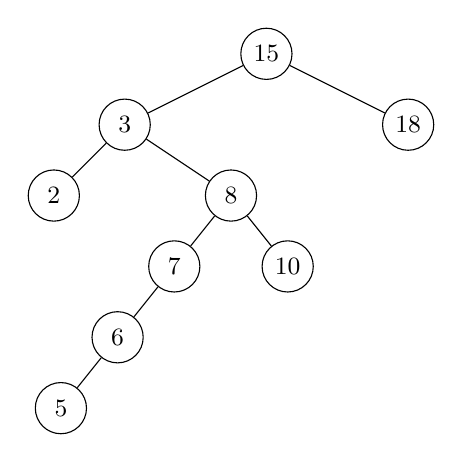
\begin{tikzpicture}[x=0.9cm, y=-0.9cm,
  v/.style={circle,draw,inner sep=0pt,minimum size=6.5mm,font=\small}]
\node[v] (15) at (4,0) {15};
\node[v] (3) at (2,1) {3};
\node[v] (18) at (6,1) {18};
\node[v] (2) at (1,2) {2};
\node[v] (8) at (3.5,2) {8};
\node[v] (7) at (2.7,3) {7};
\node[v] (10) at (4.3,3) {10};
\node[v] (6) at (1.9,4) {6};
\node[v] (5) at (1.1,5) {5};
\draw (15)--(3) (15)--(18) (3)--(2) (3)--(8) (8)--(7) (8)--(10) (7)--(6) (6)--(5);
\end{tikzpicture}
\end{center}

\textbf{(b)} 前序（根、左、右；資結書第~7.3~節）：$15$；左子樹以 $3$ 為根：$3, 2$，再以 $8$ 為根的
子樹 $8, 7, 6, 5, 10$；最後右子樹 $18$。 得到
\[
15,\ 3,\ 2,\ 8,\ 7,\ 6,\ 5,\ 10,\ 18.
\]

\textbf{(c)} Top-down 建堆積就是從空堆積開始逐一插入：新元素放在陣列最後，和父節點比，比父節點
大就交換（上浮），直到不比父節點大或到根（資結書第~8.1~節）。 每一列是插入後的陣列
（$A[1..9]$）：
\begin{center}
\begin{tabular}{lc*{9}{c}}
\toprule
操作 & 交換 & 1 & 2 & 3 & 4 & 5 & 6 & 7 & 8 & 9 \\
\midrule
插入 15 & 0 & 15 \\
插入 3 & 0 & 15 & 3 \\
插入 8 & 0 & 15 & 3 & 8 \\
插入 2 & 0 & 15 & 3 & 8 & 2 \\
插入 10 & 1 & 15 & 10 & 8 & 2 & 3 \\
插入 7 & 0 & 15 & 10 & 8 & 2 & 3 & 7 \\
插入 6 & 0 & 15 & 10 & 8 & 2 & 3 & 7 & 6 \\
插入 18 & 3 & 18 & 15 & 8 & 10 & 3 & 7 & 6 & 2 \\
插入 5 & 0 & 18 & 15 & 8 & 10 & 3 & 7 & 6 & 2 & 5 \\
\bottomrule
\end{tabular}
\end{center}
插入 $10$：放在 $A[5]$，父節點 $A[2] = 3 < 10$，交換；新的父節點 $A[1] = 15 > 10$，停。
插入 $18$：放在 $A[8]$，依序和 $A[4] = 2$、$A[2] = 10$、$A[1] = 15$ 交換，到根。 插入 $5$：放在
$A[9]$，父節點 $A[4] = 10 > 5$，不動。 結果的堆積：
\begin{center}
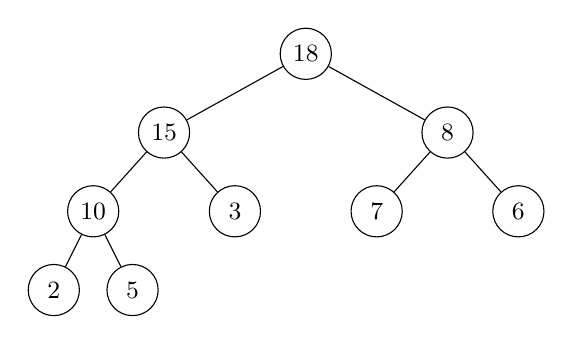
\begin{tikzpicture}[
    every node/.style={circle, draw, minimum size=6.5mm, inner sep=0pt, font=\small},
    level 1/.style={sibling distance=36mm, level distance=10mm},
    level 2/.style={sibling distance=18mm, level distance=10mm},
    level 3/.style={sibling distance=10mm, level distance=10mm}]
\node {18}
    child {node {15} child {node {10} child {node {2}} child {node {5}}} child {node {3}}}
    child {node {8} child {node {7}} child {node {6}}};
\end{tikzpicture}
\end{center}

\textbf{(d)} 堆積排序（資結書第~14.6~節、虛擬碼~14.13）：每一輪把根（目前最大）和堆積的最後一個
元素交換，堆積大小減 $1$，再把新的根下沉（和較大的子節點交換，直到不比子節點小）。 每一列是
該輪做完的陣列，直線右邊是已經排好的部分：
\begin{center}
\begin{tabular}{cll}
\toprule
輪 & 交換、下沉 & 陣列 \\
\midrule
0 & （(c) 的堆積） & $18, 15, 8, 10, 3, 7, 6, 2, 5$ \\
1 & $18 \leftrightarrow 5$；$5$ 和 $15$、$10$ 交換 & $15, 10, 8, 5, 3, 7, 6, 2 \mid 18$ \\
2 & $15 \leftrightarrow 2$；$2$ 和 $10$、$5$ 交換 & $10, 5, 8, 2, 3, 7, 6 \mid 15, 18$ \\
3 & $10 \leftrightarrow 6$；$6$ 和 $8$、$7$ 交換 & $8, 5, 7, 2, 3, 6 \mid 10, 15, 18$ \\
4 & $8 \leftrightarrow 6$；$6$ 和 $7$ 交換 & $7, 5, 6, 2, 3 \mid 8, 10, 15, 18$ \\
5 & $7 \leftrightarrow 3$；$3$ 和 $6$ 交換 & $6, 5, 3, 2 \mid 7, 8, 10, 15, 18$ \\
6 & $6 \leftrightarrow 2$；$2$ 和 $5$ 交換 & $5, 2, 3 \mid 6, 7, 8, 10, 15, 18$ \\
7 & $5 \leftrightarrow 3$；$3 > 2$，不動 & $3, 2 \mid 5, 6, 7, 8, 10, 15, 18$ \\
8 & $3 \leftrightarrow 2$ & $2 \mid 3, 5, 6, 7, 8, 10, 15, 18$ \\
\bottomrule
\end{tabular}
\end{center}
以第 1 輪為例：交換後 $A[1] = 5$，子節點 $15, 8$，和較大的 $15$ 交換；在 $A[2]$ 的子節點
$10, 3$，和 $10$ 交換；到了 $A[4]$，子節點只剩 $A[8] = 2$（$A[9]$ 已不在堆積裡），$5 > 2$，停。

由小到大的結果是 $2, 3, 5, 6, 7, 8, 10, 15, 18$。
\end{pastsoln}
